\documentclass[11pt,a4paper]{article}

% Encoding and fonts
\usepackage[utf8]{inputenc}
\usepackage[T1]{fontenc}

% Page layout
\usepackage[margin=1in]{geometry}
\usepackage{setspace}
\onehalfspacing

% Math & graphics
\usepackage{amsmath, amssymb}
\usepackage{graphicx}
\usepackage{booktabs}      % Better tables
\usepackage{caption}
\usepackage{subcaption}
\usepackage{pgfplots}      % Charts and plots
\pgfplotsset{compat=1.17}
\usepackage{pgfplotstable}
% Hyperlinks
\usepackage[hidelinks]{hyperref}

% Metadata
\title{GAN Implementation}
\author{Matthew Evans}
\date{\today}

\begin{document}

\maketitle



\section{Implementation}
We implemented a Generative Adversarial Network (GAN) in PyTorch to generate handwritten digits from the MNIST dataset. Both the generator \(G\) and the discriminator \(D\) are designed as multilayer perceptrons (MLPs). Training uses binary cross‐entropy as the loss function, and all input images are normalized with a mean of 0.5 and a standard deviation of 0.5.

\subsection{Network Architecture}
\begin{itemize}
    \item Discriminator
          \begin{enumerate}
              \item \(28\times28\) image input \(\to\) 1024 units, Leaky ReLU (negative slope 0.2)
              \item Dropout (p=0.3)
              \item 1024 \(\to\) 512 units, Leaky ReLU (0.2)
              \item Dropout (p=0.3)
              \item 512 \(\to\) 256 units, Leaky ReLU (0.2)
              \item Dropout (p=0.3)
              \item 256 \(\to\) 1 unit, Sigmoid
          \end{enumerate}
    \item Generator
          \begin{enumerate}
              \item 256 input \(\to\) 512 units, Leaky ReLU (0.2)
              \item 512 \(\to\) 1024 units, Leaky ReLU (0.2)
              \item 1024 \(\to\) \(28\times28\) output, Tanh
          \end{enumerate}
\end{itemize}

\subsection{Hyperparameters}
\begin{itemize}
    \item Dropout: 0.3
    \item Leaky ReLU negative slope: 0.2
    \item Size of \(Z\): 100
    \item Batch size: 100
    \item Learning rate: 0.0002
    \item Epochs: 200
\end{itemize}

\section{Results}

An inversion of the loss covers occurs around epoch 40. The \(D\) loss approaches \(\log(4)\) and \(G\)'s loss approaches \(-\log(\frac{1}{2})\).

This implementation uses BCE loss, which computes
\[
    -\mathbb{E}[y \log p + (1-y) \log (1-p)].
\]

At equilibrium, the optimal discriminator is \(D^*(x) = \frac{1}{2}\), so its minimax value is
\[
    V(D^*, G^*) = \log(\frac{1}{2}) + \log(\frac{1}{2}) = -\log(4) \approx -1.386.
\]

At \(D(G(z)) = \frac{1}{2}\), we have
\[
    -\log(1 - \frac{1}{2}) = -log(\frac{1}{2}) \approx 0.693.
\]

\noindent
Comfortingly, our results approach these theoretical results, as shown in table \ref{tab:loss-results} and figure \ref{fig:loss-curves}.

\begin{table}[ht]
    \centering
    \caption{Training loss by epoch and batch}
    \pgfplotstabletypeset[
        col sep=comma, % Specify that the columns are separated by commas
        header=true,   % Use the first row as the header
        % columns/Model/.style={string type}, % Ensure the "Model" column is treated as text
        every head row/.style={before row=\toprule, after row=\midrule},
        every last row/.style={after row=\bottomrule}
    ]{results-per-10-epochs.csv} % Path to your CSV file
    \label{tab:loss-results}
\end{table}

\begin{figure}[ht]
    \centering
    \begin{tikzpicture}
        \begin{axis}[
                width=0.8\linewidth,
                height=0.5\linewidth,
                xlabel=Epoch,
                ylabel=Loss,
                legend pos=north east,
                grid=major,
                grid style={dashed,gray!30},
                ymin=0,
                ymax=5,
                xmin=0,
                xmax=200
            ]
            \addplot[blue, thick] table [x=Epoch, y=D Loss, col sep=comma] {results-all.csv};
            \addlegendentry{D Loss}


            \addplot[red, thick] table [x=Epoch, y=G Loss, col sep=comma] {results-all.csv};
            \addlegendentry{D Loss}

            \addplot[black, dashed, thick] coordinates {(0,{ln(4)}) (200,{ln(4)})};
            \addlegendentry{\(\log(4)\)}

            \addplot[black, densely dotted, thick] coordinates {(0,{-ln(0.5)}) (200,{-ln(0.5)})};
            \addlegendentry{\(-\log(\frac{1}{2})\)}

        \end{axis}
    \end{tikzpicture}
    \caption{Training and validation loss curves over epochs.}
    \label{fig:loss-curves}
\end{figure}

\begin{figure}[ht]
    \centering
    % First row
    \begin{subfigure}[b]{0.48\textwidth}
        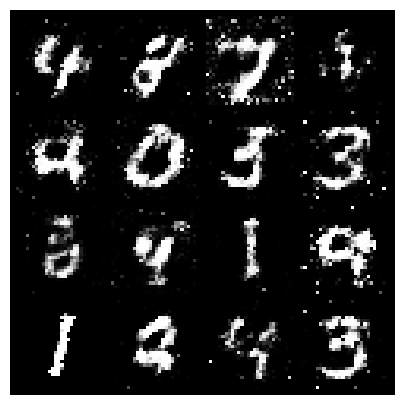
\includegraphics[width=\linewidth]{./images/epoch_25.png}
        \caption{Epoch 25}
        \label{fig:img1}
    \end{subfigure}
    \hfill
    \begin{subfigure}[b]{0.48\textwidth}
        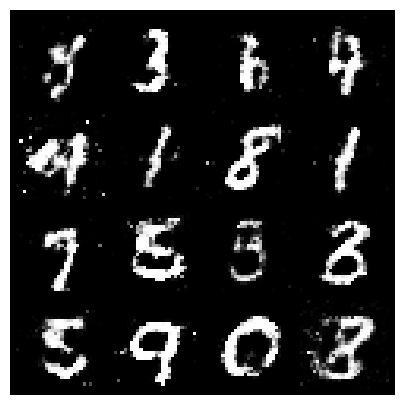
\includegraphics[width=\linewidth]{./images/epoch_50.png}
        \caption{Epoch 50}
        \label{fig:img2}
    \end{subfigure}

    \vspace{1em}

    % Second row
    \begin{subfigure}[b]{0.48\textwidth}
        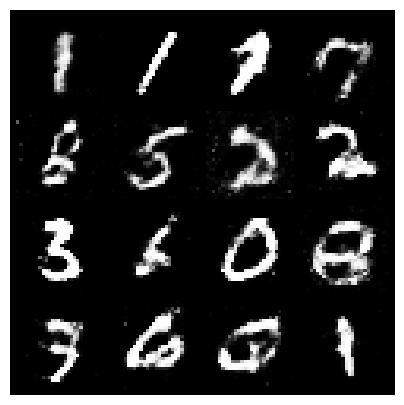
\includegraphics[width=\linewidth]{./images/epoch_100.png}
        \caption{Epoch 100}
        \label{fig:img3}
    \end{subfigure}
    \hfill
    \begin{subfigure}[b]{0.48\textwidth}
        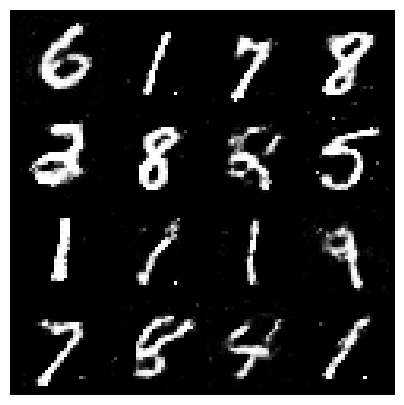
\includegraphics[width=\linewidth]{./images/epoch_200.png}
        \caption{Epoch 200}
        \label{fig:img4}
    \end{subfigure}

    \caption{Generated samples at different epochs in the learning process.}
    \label{fig:2x2grid}
\end{figure}

\bibliographystyle{plain}
\bibliography{references}

\end{document}